\begin{figure*}[t]
\centering
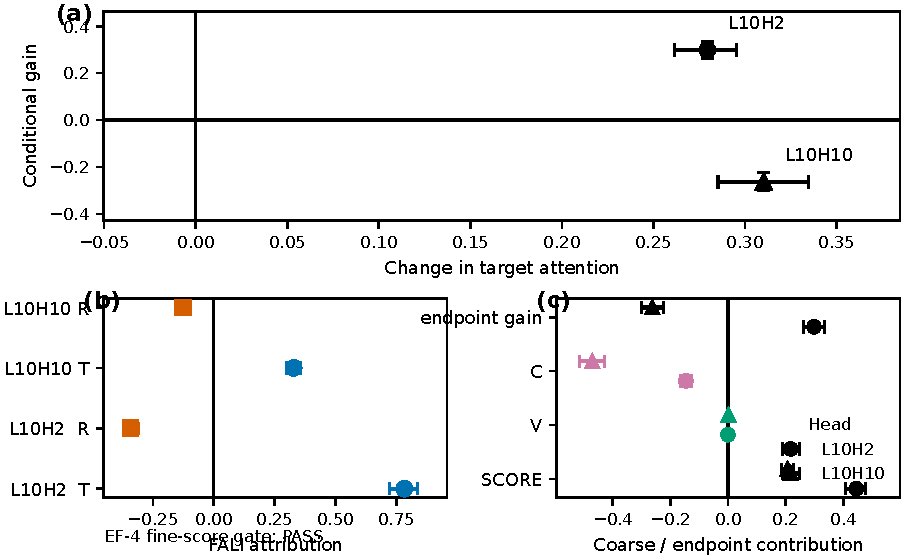
\includegraphics[width=\textwidth]{figures/Fig4.pdf}
\caption{\textbf{Target-attention adaptation and positive functional recruitment are distinct in GPT-2 IOI.}
(a) L10H2 and L10H10 both increase attention to the IO target after the canonical primary Name Movers are ablated, but their conditional gains have opposite signs: L10H2 becomes more causally useful whereas L10H10 becomes less useful on the broad canonical distribution.
(b) Both heads nevertheless show positive target-score and negative rival-score FALI contributions under the preregistered confirmatory analysis.
(c) Coarse attribution clarifies the distinction: L10H10's positive SCORE contribution is outweighed by a substantially negative surrounding-context contribution, producing a negative endpoint change.
Points are exact balanced means; intervals are hierarchical 95\% bootstrap CIs over the canonical template design.}
\label{fig:gpt2-attention-recruitment}
\end{figure*}
